\chapter{Gestión de residuos sólidos}
\label{chap2}
\ifpdf
  \graphicspath{{Chapter2/Chapter2Figs/}}
\else
  \graphicspath{{Chapter2/Chapter2Figs/}}\fi

\markboth{\hfill \thechapter. Gestión de residuos sólidos}{\hfill \thechapter. Gestión de residuos sólidos}

La gestión de residuos sólidos (SWM, \textit{Solid Waste Management}) implica varios procesos que pueden dar lugar a problemas relacionados con áreas como la organización, el control, la logística, la planificación y el reciclaje. Es una actividad multidisciplinaria que contiene decisiones de criterios múltiples en cada etapa de su ciclo de vida. Existen investigaciones en varios aspectos, como el área de pronóstico de generación de residuos, el monitoreo de los sistemas de recolección de contenedores, la gestión del transporte de contenedores y la predicción de la instalación de nuevas plantas de eliminación de residuos. \citep{VitorinodeSouzaMelare2017TechnologiesReview}

\citet{VitorinodeSouzaMelare2017TechnologiesReview} agrupa los procesos de SWM en seis categorías. 
\begin{itemize}
\item La gestión de recogida, recorrido y transporte; 
\item Gestión y seguimiento de contenedores; 
\item Reciclaje de residuos sólidos y gestión de residuos electrónicos; 
\item Administración pública y desarrollo sostenible; 
\item Métodos de previsión y planificación; y 
\item Determinación de sitios de disposición de residuos.
\end{itemize}


Según \citet{Acurio1997DiagnosticoCaribe}, los residuos sólidos urbanos se pueden clasificar en:
\begin{itemize}
\item \textbf{Residuos sólidos municipales (RSM):} Los residuos sólidos municipales son aquellos provenientes de la generación residencial, comercial, institucional, industrial (pequeña industria y artesanía) y los residuos sólidos resultantes del barrido de calles de un conglomerado urbano y cuya gestión está a cargo de las autoridades municipales.
\item \textbf{Residuos sólidos especiales (RSE):} Algunos de los residuos especiales por su cantidad o manejo pueden presentar un riesgo a la salud, tales como los residuos sólidos provenientes de establecimientos de salud; los productos químicos y fármacos caducos.
\item \textbf{Residuos peligrosos (RP):} Los residuos peligrosos son aquellos sólidos o semisólidos que por sus características tóxicas, reactivas, corrosivas, radiactivas, inflamables o infecciosas plantean un riesgo sustancial real o potencial a la salud humana o al medio ambiente.
\end{itemize}

% \section{Antecedente}
\section{Gestión de residuos sólidos en la ciudad de Asunción}

Asunción es la capital y la ciudad más poblada de la República del Paraguay. Es un municipio autónomo administrado como Distrito capital y no forma parte formalmente de ningún departamento, cuenta con una superficie de 117 km2, dividido actualmente en 68 barrios. Según las proyecciones de la \citet*{DireccionGeneraldeEstadistica2015Paraguay2000-2025} para el año 2017 estiman una población aproximada de 524.190 habitantes. Se debe agregar que el ingreso promedio de  personas en ómnibus del transporte público y vehículos privados de los municipios aledaños, es alrededor de 1.320.000 a diario. Este análisis se hace en base a cálculos estimativos de la Unidad Coordinadora del Programa Metrobús del MOPC \citep{DiarioABCColor2016PorColor}. La cantidad de personas que convergen diariamente en Asunción trae consigo una alta generación de residuos, esto hace que la complejidad en la gestión de los mismos sea cada vez mayor.

La Dirección de Servicios Urbanos de la ciudad de Asunción es la encargada de la regulación y prestación de servicios de aseo, de recolección, disposición y tratamiento de los residuos del municipio, así como también del equipamiento, mantenimiento, limpieza y ornato de la infraestructura pública del municipio, incluyendo las calles, avenidas, parques, plazas, balnearios y demás lugares públicos. Según Rodrigo Velázquez, director de la DSU, el promedio diario normal de basura recogida suele ser entre 800.000 y 900.000 kilos \citep{LaNacion2016AsuncionBasura} [Dato obtenido en 9 de Enero de 2016]. 
% El Dato obtenido tiene la fecha de la publicacion en el diario, no la fecha de acceso
%Se tiene la cantidad exacta de zonas ahora
Actualmente el Departamento de Recolección de la DSU es la responsable de la recolección de residuos sólidos, para ello divide la ciudad en zonas, según datos brindados por la DSU en el 2010 la ciudad estaba dividida en 120, como se muestra en la figura \ref{fig:zonasRecoleccion}. La DSU cuenta con contenedores medianos y grandes distribuidos por todo el municipio, estos son tratados de la misma manera que los residuos domiciliarios, como mínimo debe existir una calle empedrada para que los vehículos recojan los residuos, es por esto que lugares como "El Bañado Norte y Sur" no son beneficiados con el servicio.

\subsection{Procedimiento de recolección de la basura en la Municipalidad de Asunción}

A continuación se detalla el procedimiento llevado a cabo habitualmente para la recolección de la basura:

\begin{itemize}
\item Cada zona es asignada a un vehículo recolector de basura.
\item Cada vehículo cuenta con un chofer y dos ayudantes, y es identificado por su chapa o por el número que fue asignado por la DSU. Estos vehículos recolectores son de propiedad de la Municipalidad de Asunción, y cuando uno de ellos queda fuera de servicio por algún desperfecto, por lo general, la solución radica en alquilar un recolector para que lo cubra.
\item Todas las unidades depositan la basura en el vertedero que se encuentra en Cateura, donde no existe una diferenciación de los residuos recolectados, por su parte, los residuos hospitalarios son recolectados por una empresa tercerizada por el municipio y no son depositados en Cateura.
\item El vehículo recolector inicia su recorrido cuando sale de la DSU en dirección a su zona.
\item Luego de haber recogido toda la basura domiciliaria de la zona, el vehículo se dirige al vertedero para depositar los residuos y de allí vuelve a su punto de partida. Generalmente, el vehículo tiene capacidad suficiente para realizar un solo viaje de su zona al vertedero, pero si no es el caso, debe realizar la cantidad de viajes necesarios hasta recolectar todos los residuos domiciliarios de la zona en cuestión.
\item El servicio de recolección domiciliaria se realiza de lunes a sábados, y se divide en 3 turnos: mañana, tarde y noche, donde cada turno tiene una duración máxima de 6 horas.
\end{itemize}

\begin{figure}[H]
    \centering
    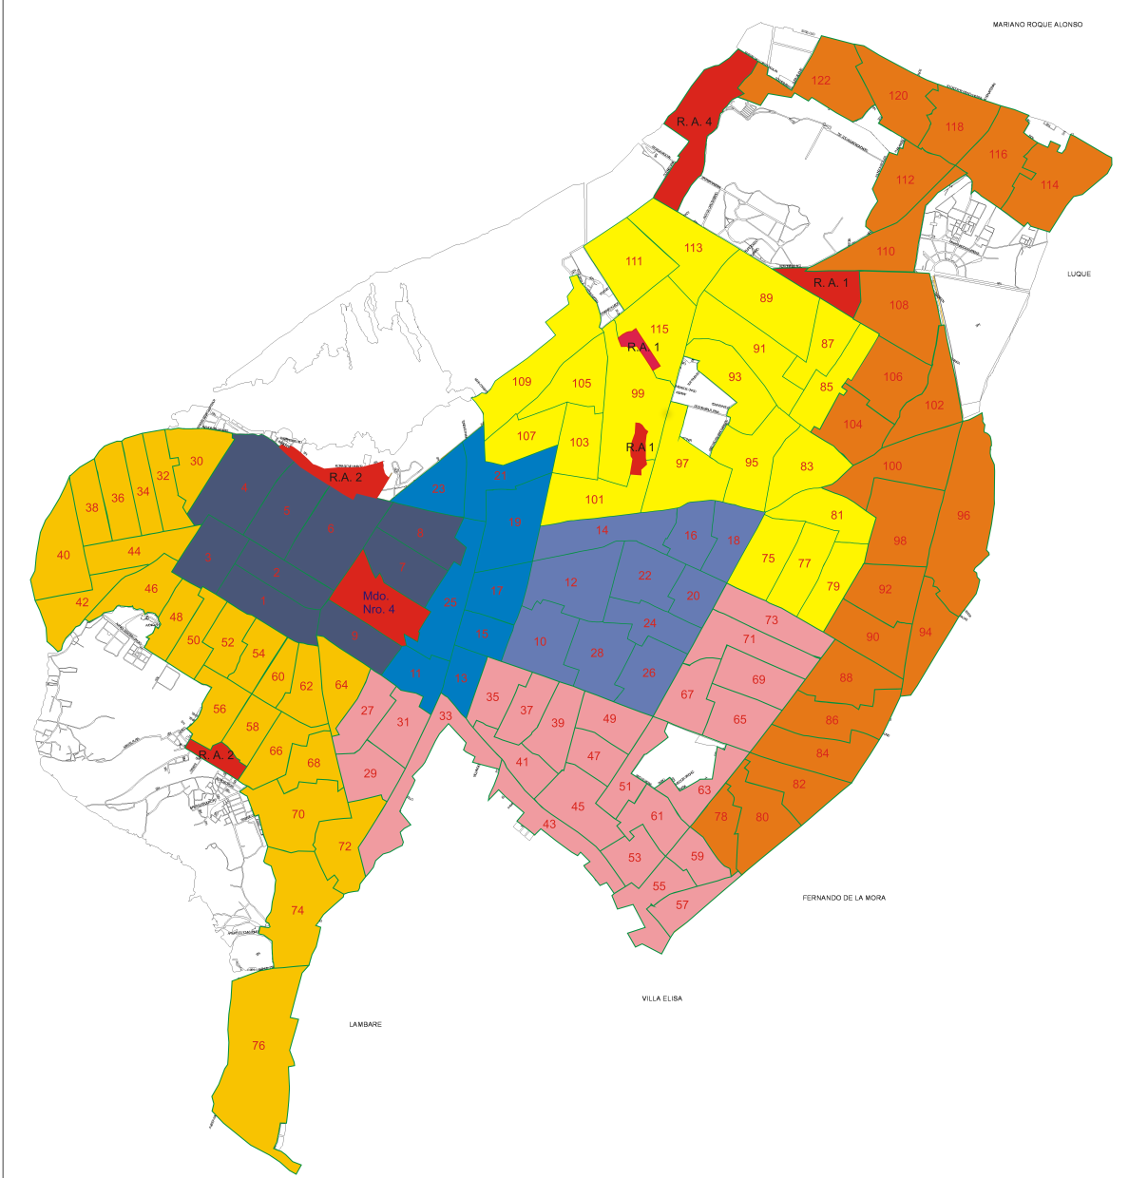
\includegraphics[width=4.5cm]{Recoleccion-ZONAS&CUADRANTES.png}
    \caption{División de la ciudad en zonas. Un turno en el mapa está correspondido por un conjunto de zonas coloreadas del mismo color. [Fuente: Departamento de Recolección de la DSU]}
    \label{fig:zonasRecoleccion}
\end{figure}

En la figura \ref{fig:zonasRecoleccion}, un turno se corresponde con un conjunto de zonas, las zonas pintadas en azul oscuro, correspondientes al microcentro, tienen un tratamiento especial ya que son las únicas zonas que son atendidas todos los días. Los residuos en estas zonas son recolectados en el turno noche debido al poco tráfico registrado en esas calles en comparación a cualquier otro turno. Las zonas no pintadas no tienen número, y por ende no son cubiertas por el servicio, sin embargo representan una zona candidata a futuro para recolección de la basura.